% Created by tikzDevice version 0.12.6 on 2024-02-19 10:08:23
% !TEX encoding = UTF-8 Unicode
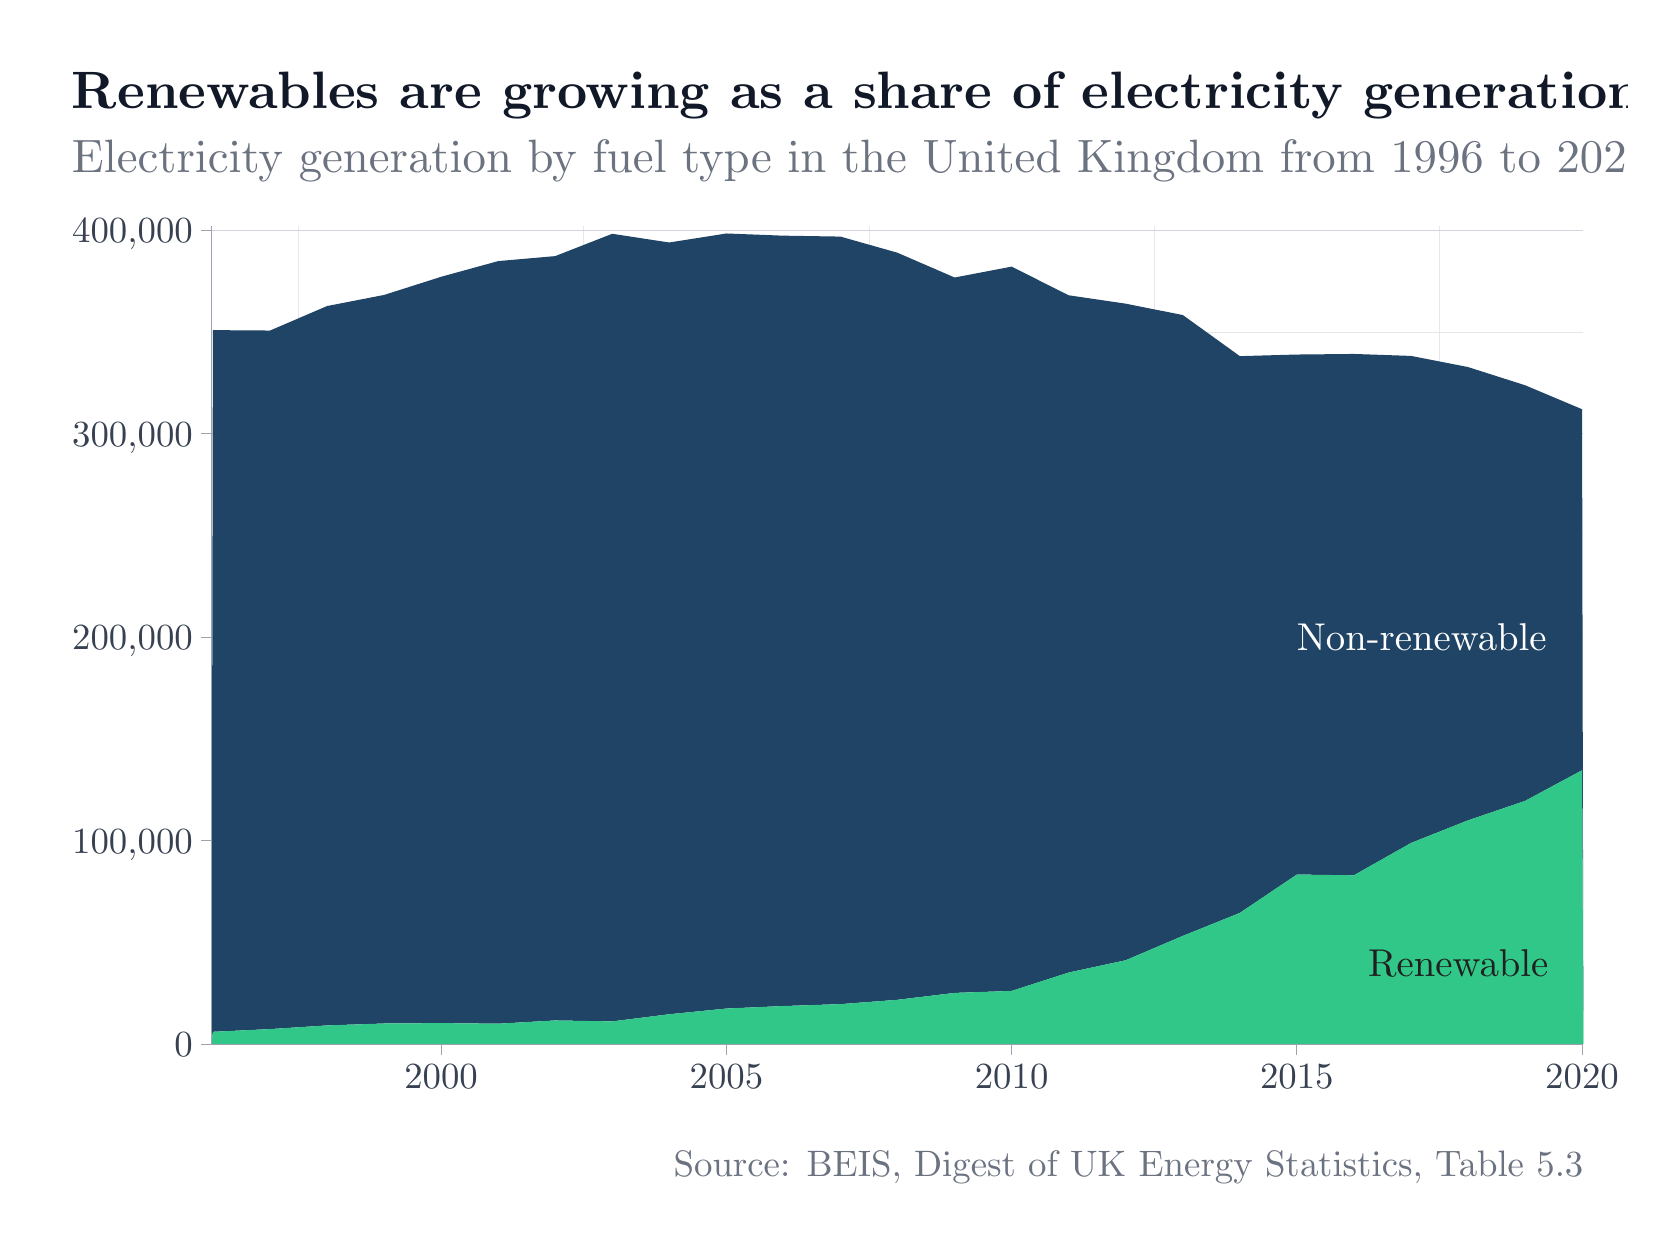
\begin{tikzpicture}[x=1pt,y=1pt]
\definecolor{fillColor}{RGB}{255,255,255}
\path[use as bounding box,fill=fillColor] (0,0) rectangle (578.16,433.62);
\begin{scope}
\path[clip] (  0.00,  0.00) rectangle (578.16,433.62);
\definecolor{drawColor}{RGB}{255,255,255}

\path[draw=drawColor,line width= 0.8pt,line join=round,line cap=round,fill=fillColor] (  0.00,  0.00) rectangle (578.16,433.62);
\end{scope}
\begin{scope}
\path[clip] ( 66.43, 66.29) rectangle (562.16,361.93);
\definecolor{drawColor}{RGB}{255,255,255}
\definecolor{fillColor}{RGB}{255,255,255}

\path[draw=drawColor,line width= 0.8pt,line join=round,line cap=round,fill=fillColor] ( 66.43, 66.29) rectangle (562.16,361.93);
\definecolor{drawColor}{RGB}{229,231,235}

\path[draw=drawColor,line width= 0.2pt,line join=round] ( 66.43,103.06) --
	(562.16,103.06);

\path[draw=drawColor,line width= 0.2pt,line join=round] ( 66.43,176.60) --
	(562.16,176.60);

\path[draw=drawColor,line width= 0.2pt,line join=round] ( 66.43,250.14) --
	(562.16,250.14);

\path[draw=drawColor,line width= 0.2pt,line join=round] ( 66.43,323.68) --
	(562.16,323.68);

\path[draw=drawColor,line width= 0.2pt,line join=round] ( 97.83, 66.29) --
	( 97.83,361.93);

\path[draw=drawColor,line width= 0.2pt,line join=round] (200.94, 66.29) --
	(200.94,361.93);

\path[draw=drawColor,line width= 0.2pt,line join=round] (304.02, 66.29) --
	(304.02,361.93);

\path[draw=drawColor,line width= 0.2pt,line join=round] (407.08, 66.29) --
	(407.08,361.93);

\path[draw=drawColor,line width= 0.2pt,line join=round] (510.14, 66.29) --
	(510.14,361.93);
\definecolor{drawColor}{RGB}{209,213,219}

\path[draw=drawColor,line width= 0.4pt,line join=round] ( 66.43, 66.29) --
	(562.16, 66.29);

\path[draw=drawColor,line width= 0.4pt,line join=round] ( 66.43,139.83) --
	(562.16,139.83);

\path[draw=drawColor,line width= 0.4pt,line join=round] ( 66.43,213.37) --
	(562.16,213.37);

\path[draw=drawColor,line width= 0.4pt,line join=round] ( 66.43,286.91) --
	(562.16,286.91);

\path[draw=drawColor,line width= 0.4pt,line join=round] ( 66.43,360.45) --
	(562.16,360.45);
\definecolor{fillColor}{RGB}{32,68,102}

\path[fill=fillColor] ( 66.93,324.32) --
	( 67.42,324.32) --
	( 87.09,324.18) --
	( 87.58,324.17) --
	( 88.08,324.39) --
	(107.69,332.81) --
	(108.18,333.03) --
	(108.68,333.12) --
	(128.29,336.94) --
	(128.78,337.03) --
	(129.28,337.19) --
	(148.89,343.43) --
	(149.38,343.59) --
	(149.88,343.73) --
	(169.54,349.13) --
	(170.04,349.27) --
	(170.53,349.31) --
	(190.14,351.03) --
	(190.64,351.07) --
	(191.13,351.27) --
	(210.74,358.94) --
	(211.24,359.14) --
	(211.73,359.06) --
	(231.34,356.06) --
	(231.84,355.99) --
	(232.33,356.07) --
	(252.00,359.17) --
	(252.50,359.25) --
	(252.99,359.23) --
	(272.60,358.47) --
	(273.10,358.46) --
	(273.59,358.45) --
	(293.20,358.13) --
	(293.70,358.12) --
	(294.19,357.98) --
	(313.80,352.43) --
	(314.30,352.29) --
	(314.79,352.07) --
	(334.46,343.55) --
	(334.95,343.33) --
	(335.45,343.43) --
	(355.06,347.17) --
	(355.55,347.27) --
	(356.05,347.02) --
	(375.66,337.16) --
	(376.15,336.91) --
	(376.65,336.84) --
	(396.26,333.96) --
	(396.75,333.89) --
	(397.25,333.79) --
	(416.91,329.87) --
	(417.41,329.78) --
	(417.90,329.42) --
	(437.51,315.29) --
	(438.01,314.93) --
	(438.50,314.94) --
	(458.11,315.49) --
	(458.61,315.50) --
	(459.10,315.51) --
	(478.71,315.71) --
	(479.21,315.72) --
	(479.70,315.70) --
	(499.37,315.02) --
	(499.87,315.00) --
	(500.36,314.91) --
	(519.97,311.08) --
	(520.47,310.98) --
	(520.96,310.82) --
	(540.57,304.57) --
	(541.07,304.42) --
	(541.56,304.21) --
	(561.17,295.95) --
	(561.67,295.74) --
	(562.16, 66.29) --
	(561.67,165.28) --
	(561.17,165.02) --
	(541.56,154.47) --
	(541.07,154.20) --
	(540.57,154.04) --
	(520.96,147.35) --
	(520.47,147.18) --
	(519.97,146.99) --
	(500.36,139.21) --
	(499.87,139.01) --
	(499.37,138.73) --
	(479.70,127.61) --
	(479.21,127.33) --
	(478.71,127.33) --
	(459.10,127.59) --
	(458.61,127.60) --
	(458.11,127.27) --
	(438.50,114.08) --
	(438.01,113.74) --
	(437.51,113.54) --
	(417.90,105.63) --
	(417.41,105.43) --
	(416.91,105.22) --
	(397.25, 96.84) --
	(396.75, 96.63) --
	(396.26, 96.52) --
	(376.65, 92.30) --
	(376.15, 92.19) --
	(375.66, 92.03) --
	(356.05, 85.71) --
	(355.55, 85.55) --
	(355.06, 85.53) --
	(335.45, 84.85) --
	(334.95, 84.83) --
	(334.46, 84.77) --
	(314.79, 82.40) --
	(314.30, 82.34) --
	(313.80, 82.30) --
	(294.19, 80.81) --
	(293.70, 80.77) --
	(293.20, 80.76) --
	(273.59, 80.10) --
	(273.10, 80.09) --
	(272.60, 80.07) --
	(252.99, 79.20) --
	(252.50, 79.18) --
	(252.00, 79.13) --
	(232.33, 77.17) --
	(231.84, 77.12) --
	(231.34, 77.06) --
	(211.73, 74.60) --
	(211.24, 74.54) --
	(210.74, 74.54) --
	(191.13, 74.87) --
	(190.64, 74.88) --
	(190.14, 74.85) --
	(170.53, 73.73) --
	(170.04, 73.70) --
	(169.54, 73.71) --
	(149.88, 73.91) --
	(149.38, 73.91) --
	(148.89, 73.91) --
	(129.28, 73.78) --
	(128.78, 73.78) --
	(128.29, 73.76) --
	(108.68, 73.10) --
	(108.18, 73.08) --
	(107.69, 73.05) --
	( 88.08, 71.79) --
	( 87.58, 71.76) --
	( 87.09, 71.73) --
	( 67.42, 70.80) --
	( 66.93, 70.78) --
	( 66.43, 66.29) --
	cycle;

\path[] ( 66.93,324.32) --
	( 67.42,324.32) --
	( 87.09,324.18) --
	( 87.58,324.17) --
	( 88.08,324.39) --
	(107.69,332.81) --
	(108.18,333.03) --
	(108.68,333.12) --
	(128.29,336.94) --
	(128.78,337.03) --
	(129.28,337.19) --
	(148.89,343.43) --
	(149.38,343.59) --
	(149.88,343.73) --
	(169.54,349.13) --
	(170.04,349.27) --
	(170.53,349.31) --
	(190.14,351.03) --
	(190.64,351.07) --
	(191.13,351.27) --
	(210.74,358.94) --
	(211.24,359.14) --
	(211.73,359.06) --
	(231.34,356.06) --
	(231.84,355.99) --
	(232.33,356.07) --
	(252.00,359.17) --
	(252.50,359.25) --
	(252.99,359.23) --
	(272.60,358.47) --
	(273.10,358.46) --
	(273.59,358.45) --
	(293.20,358.13) --
	(293.70,358.12) --
	(294.19,357.98) --
	(313.80,352.43) --
	(314.30,352.29) --
	(314.79,352.07) --
	(334.46,343.55) --
	(334.95,343.33) --
	(335.45,343.43) --
	(355.06,347.17) --
	(355.55,347.27) --
	(356.05,347.02) --
	(375.66,337.16) --
	(376.15,336.91) --
	(376.65,336.84) --
	(396.26,333.96) --
	(396.75,333.89) --
	(397.25,333.79) --
	(416.91,329.87) --
	(417.41,329.78) --
	(417.90,329.42) --
	(437.51,315.29) --
	(438.01,314.93) --
	(438.50,314.94) --
	(458.11,315.49) --
	(458.61,315.50) --
	(459.10,315.51) --
	(478.71,315.71) --
	(479.21,315.72) --
	(479.70,315.70) --
	(499.37,315.02) --
	(499.87,315.00) --
	(500.36,314.91) --
	(519.97,311.08) --
	(520.47,310.98) --
	(520.96,310.82) --
	(540.57,304.57) --
	(541.07,304.42) --
	(541.56,304.21) --
	(561.17,295.95) --
	(561.67,295.74);
\definecolor{fillColor}{RGB}{48,199,136}

\path[fill=fillColor] ( 66.93, 70.78) --
	( 67.42, 70.80) --
	( 87.09, 71.73) --
	( 87.58, 71.76) --
	( 88.08, 71.79) --
	(107.69, 73.05) --
	(108.18, 73.08) --
	(108.68, 73.10) --
	(128.29, 73.76) --
	(128.78, 73.78) --
	(129.28, 73.78) --
	(148.89, 73.91) --
	(149.38, 73.91) --
	(149.88, 73.91) --
	(169.54, 73.71) --
	(170.04, 73.70) --
	(170.53, 73.73) --
	(190.14, 74.85) --
	(190.64, 74.88) --
	(191.13, 74.87) --
	(210.74, 74.54) --
	(211.24, 74.54) --
	(211.73, 74.60) --
	(231.34, 77.06) --
	(231.84, 77.12) --
	(232.33, 77.17) --
	(252.00, 79.13) --
	(252.50, 79.18) --
	(252.99, 79.20) --
	(272.60, 80.07) --
	(273.10, 80.09) --
	(273.59, 80.10) --
	(293.20, 80.76) --
	(293.70, 80.77) --
	(294.19, 80.81) --
	(313.80, 82.30) --
	(314.30, 82.34) --
	(314.79, 82.40) --
	(334.46, 84.77) --
	(334.95, 84.83) --
	(335.45, 84.85) --
	(355.06, 85.53) --
	(355.55, 85.55) --
	(356.05, 85.71) --
	(375.66, 92.03) --
	(376.15, 92.19) --
	(376.65, 92.30) --
	(396.26, 96.52) --
	(396.75, 96.63) --
	(397.25, 96.84) --
	(416.91,105.22) --
	(417.41,105.43) --
	(417.90,105.63) --
	(437.51,113.54) --
	(438.01,113.74) --
	(438.50,114.08) --
	(458.11,127.27) --
	(458.61,127.60) --
	(459.10,127.59) --
	(478.71,127.33) --
	(479.21,127.33) --
	(479.70,127.61) --
	(499.37,138.73) --
	(499.87,139.01) --
	(500.36,139.21) --
	(519.97,146.99) --
	(520.47,147.18) --
	(520.96,147.35) --
	(540.57,154.04) --
	(541.07,154.20) --
	(541.56,154.47) --
	(561.17,165.02) --
	(561.67,165.28) --
	(562.16, 66.29) --
	(561.67, 66.29) --
	(561.17, 66.29) --
	(541.56, 66.29) --
	(541.07, 66.29) --
	(540.57, 66.29) --
	(520.96, 66.29) --
	(520.47, 66.29) --
	(519.97, 66.29) --
	(500.36, 66.29) --
	(499.87, 66.29) --
	(499.37, 66.29) --
	(479.70, 66.29) --
	(479.21, 66.29) --
	(478.71, 66.29) --
	(459.10, 66.29) --
	(458.61, 66.29) --
	(458.11, 66.29) --
	(438.50, 66.29) --
	(438.01, 66.29) --
	(437.51, 66.29) --
	(417.90, 66.29) --
	(417.41, 66.29) --
	(416.91, 66.29) --
	(397.25, 66.29) --
	(396.75, 66.29) --
	(396.26, 66.29) --
	(376.65, 66.29) --
	(376.15, 66.29) --
	(375.66, 66.29) --
	(356.05, 66.29) --
	(355.55, 66.29) --
	(355.06, 66.29) --
	(335.45, 66.29) --
	(334.95, 66.29) --
	(334.46, 66.29) --
	(314.79, 66.29) --
	(314.30, 66.29) --
	(313.80, 66.29) --
	(294.19, 66.29) --
	(293.70, 66.29) --
	(293.20, 66.29) --
	(273.59, 66.29) --
	(273.10, 66.29) --
	(272.60, 66.29) --
	(252.99, 66.29) --
	(252.50, 66.29) --
	(252.00, 66.29) --
	(232.33, 66.29) --
	(231.84, 66.29) --
	(231.34, 66.29) --
	(211.73, 66.29) --
	(211.24, 66.29) --
	(210.74, 66.29) --
	(191.13, 66.29) --
	(190.64, 66.29) --
	(190.14, 66.29) --
	(170.53, 66.29) --
	(170.04, 66.29) --
	(169.54, 66.29) --
	(149.88, 66.29) --
	(149.38, 66.29) --
	(148.89, 66.29) --
	(129.28, 66.29) --
	(128.78, 66.29) --
	(128.29, 66.29) --
	(108.68, 66.29) --
	(108.18, 66.29) --
	(107.69, 66.29) --
	( 88.08, 66.29) --
	( 87.58, 66.29) --
	( 87.09, 66.29) --
	( 67.42, 66.29) --
	( 66.93, 66.29) --
	( 66.43, 66.29) --
	cycle;

\path[] ( 66.93, 70.78) --
	( 67.42, 70.80) --
	( 87.09, 71.73) --
	( 87.58, 71.76) --
	( 88.08, 71.79) --
	(107.69, 73.05) --
	(108.18, 73.08) --
	(108.68, 73.10) --
	(128.29, 73.76) --
	(128.78, 73.78) --
	(129.28, 73.78) --
	(148.89, 73.91) --
	(149.38, 73.91) --
	(149.88, 73.91) --
	(169.54, 73.71) --
	(170.04, 73.70) --
	(170.53, 73.73) --
	(190.14, 74.85) --
	(190.64, 74.88) --
	(191.13, 74.87) --
	(210.74, 74.54) --
	(211.24, 74.54) --
	(211.73, 74.60) --
	(231.34, 77.06) --
	(231.84, 77.12) --
	(232.33, 77.17) --
	(252.00, 79.13) --
	(252.50, 79.18) --
	(252.99, 79.20) --
	(272.60, 80.07) --
	(273.10, 80.09) --
	(273.59, 80.10) --
	(293.20, 80.76) --
	(293.70, 80.77) --
	(294.19, 80.81) --
	(313.80, 82.30) --
	(314.30, 82.34) --
	(314.79, 82.40) --
	(334.46, 84.77) --
	(334.95, 84.83) --
	(335.45, 84.85) --
	(355.06, 85.53) --
	(355.55, 85.55) --
	(356.05, 85.71) --
	(375.66, 92.03) --
	(376.15, 92.19) --
	(376.65, 92.30) --
	(396.26, 96.52) --
	(396.75, 96.63) --
	(397.25, 96.84) --
	(416.91,105.22) --
	(417.41,105.43) --
	(417.90,105.63) --
	(437.51,113.54) --
	(438.01,113.74) --
	(438.50,114.08) --
	(458.11,127.27) --
	(458.61,127.60) --
	(459.10,127.59) --
	(478.71,127.33) --
	(479.21,127.33) --
	(479.70,127.61) --
	(499.37,138.73) --
	(499.87,139.01) --
	(500.36,139.21) --
	(519.97,146.99) --
	(520.47,147.18) --
	(520.96,147.35) --
	(540.57,154.04) --
	(541.07,154.20) --
	(541.56,154.47) --
	(561.17,165.02) --
	(561.67,165.28);
\definecolor{drawColor}{RGB}{255,255,255}

\node[text=drawColor,anchor=base west,inner sep=0pt, outer sep=0pt, scale=  1.40] at (458.61,208.55) {Non-renewable};
\definecolor{drawColor}{RGB}{32,32,32}

\node[text=drawColor,anchor=base west,inner sep=0pt, outer sep=0pt, scale=  1.40] at (484.34, 90.89) {Renewable};

\path[] ( 66.43, 66.29) rectangle (562.16,361.93);
\end{scope}
\begin{scope}
\path[clip] (  0.00,  0.00) rectangle (578.16,433.62);
\definecolor{drawColor}{RGB}{156,163,175}

\path[draw=drawColor,line width= 0.3pt,line join=round] ( 66.43, 66.29) --
	( 66.43,361.93);
\end{scope}
\begin{scope}
\path[clip] (  0.00,  0.00) rectangle (578.16,433.62);
\definecolor{drawColor}{RGB}{55,65,81}

\node[text=drawColor,anchor=base east,inner sep=0pt, outer sep=0pt, scale=  1.33] at ( 59.68, 61.70) {0};

\node[text=drawColor,anchor=base east,inner sep=0pt, outer sep=0pt, scale=  1.33] at ( 59.68,135.24) {100,000};

\node[text=drawColor,anchor=base east,inner sep=0pt, outer sep=0pt, scale=  1.33] at ( 59.68,208.78) {200,000};

\node[text=drawColor,anchor=base east,inner sep=0pt, outer sep=0pt, scale=  1.33] at ( 59.68,282.32) {300,000};

\node[text=drawColor,anchor=base east,inner sep=0pt, outer sep=0pt, scale=  1.33] at ( 59.68,355.86) {400,000};
\end{scope}
\begin{scope}
\path[clip] (  0.00,  0.00) rectangle (578.16,433.62);
\definecolor{drawColor}{RGB}{156,163,175}

\path[draw=drawColor,line width= 0.3pt,line join=round] ( 62.68, 66.29) --
	( 66.43, 66.29);

\path[draw=drawColor,line width= 0.3pt,line join=round] ( 62.68,139.83) --
	( 66.43,139.83);

\path[draw=drawColor,line width= 0.3pt,line join=round] ( 62.68,213.37) --
	( 66.43,213.37);

\path[draw=drawColor,line width= 0.3pt,line join=round] ( 62.68,286.91) --
	( 66.43,286.91);

\path[draw=drawColor,line width= 0.3pt,line join=round] ( 62.68,360.45) --
	( 66.43,360.45);
\end{scope}
\begin{scope}
\path[clip] (  0.00,  0.00) rectangle (578.16,433.62);
\definecolor{drawColor}{RGB}{156,163,175}

\path[draw=drawColor,line width= 0.3pt,line join=round] ( 66.43, 66.29) --
	(562.16, 66.29);
\end{scope}
\begin{scope}
\path[clip] (  0.00,  0.00) rectangle (578.16,433.62);
\definecolor{drawColor}{RGB}{156,163,175}

\path[draw=drawColor,line width= 0.3pt,line join=round] (149.38, 62.54) --
	(149.38, 66.29);

\path[draw=drawColor,line width= 0.3pt,line join=round] (252.50, 62.54) --
	(252.50, 66.29);

\path[draw=drawColor,line width= 0.3pt,line join=round] (355.55, 62.54) --
	(355.55, 66.29);

\path[draw=drawColor,line width= 0.3pt,line join=round] (458.61, 62.54) --
	(458.61, 66.29);

\path[draw=drawColor,line width= 0.3pt,line join=round] (561.67, 62.54) --
	(561.67, 66.29);
\end{scope}
\begin{scope}
\path[clip] (  0.00,  0.00) rectangle (578.16,433.62);
\definecolor{drawColor}{RGB}{55,65,81}

\node[text=drawColor,anchor=base,inner sep=0pt, outer sep=0pt, scale=  1.33] at (149.38, 50.36) {2000};

\node[text=drawColor,anchor=base,inner sep=0pt, outer sep=0pt, scale=  1.33] at (252.50, 50.36) {2005};

\node[text=drawColor,anchor=base,inner sep=0pt, outer sep=0pt, scale=  1.33] at (355.55, 50.36) {2010};

\node[text=drawColor,anchor=base,inner sep=0pt, outer sep=0pt, scale=  1.33] at (458.61, 50.36) {2015};

\node[text=drawColor,anchor=base,inner sep=0pt, outer sep=0pt, scale=  1.33] at (561.67, 50.36) {2020};
\end{scope}
\begin{scope}
\path[clip] (  0.00,  0.00) rectangle (578.16,433.62);
\definecolor{drawColor}{RGB}{107,114,128}

\node[text=drawColor,anchor=base west,inner sep=0pt, outer sep=0pt, scale=  1.69] at ( 16.00,381.21) {Electricity generation by fuel type in the United Kingdom from 1996 to 2020, GWh};
\end{scope}
\begin{scope}
\path[clip] (  0.00,  0.00) rectangle (578.16,433.62);
\definecolor{drawColor}{RGB}{17,24,39}

\node[text=drawColor,anchor=base west,inner sep=0pt, outer sep=0pt, scale=  1.90] at ( 16.00,404.52) {\bfseries Renewables are growing as a share of electricity generation};
\end{scope}
\begin{scope}
\path[clip] (  0.00,  0.00) rectangle (578.16,433.62);
\definecolor{drawColor}{RGB}{107,114,128}

\node[text=drawColor,anchor=base east,inner sep=0pt, outer sep=0pt, scale=  1.33] at (562.16, 18.59) {Source: BEIS, Digest of UK Energy Statistics, Table 5.3};
\end{scope}
\end{tikzpicture}
